%!TEX TS-program = xelatex
%!TEX encoding = UTF-8 Unicode

\documentclass[tikz,border=1]{standalone}
\usetikzlibrary{positioning}

\begin{document}
  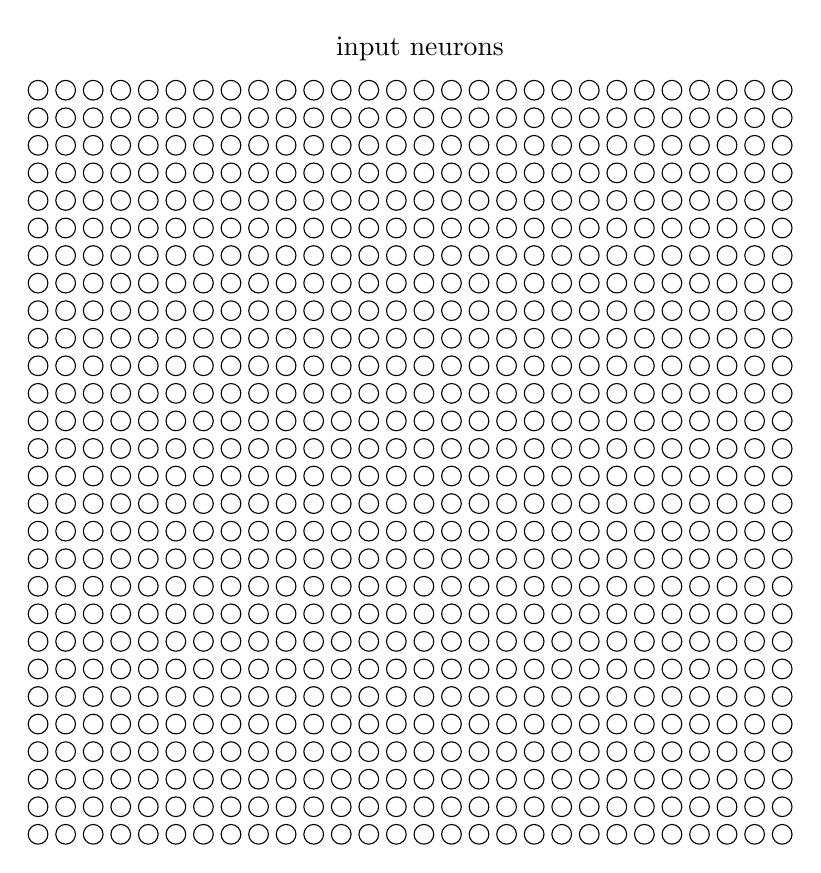
\begin{tikzpicture}[
    neuron/.style={circle,draw,inner sep=0pt,minimum size=2.5mm}
    ]

    \foreach \x in {0,...,27}
      \foreach \y in {0,...,27}
        \node (x\x{}y\y) [neuron] at (\x * 0.35,\y * 0.35) {};

    \node [above] at (4.85,9.7) {input neurons};

  \end{tikzpicture} 
\end{document}
